\documentclass{aamas2013}
\usepackage{algorithmic}
\usepackage{algorithm}

% if you are using PDF LaTex and you cannot find a way for producing
% letter, the following explicit settings may help
 
\pdfpagewidth=8.5truein
\pdfpageheight=11truein

\begin{document}

% In the original styles from ACM, you would have needed to
% add meta-info here. This is not necessary for AAMAS 2013  as
% the complete copyright information is generated by the cls-files.


\title{Novel Approaches for Exploiting Opponents in Poker}

\numberofauthors{1}

\author{
% 1st. author
\alignauthor
%Paper  XXX
Wesley Tansey\\
       \affaddr{University of Texas at Austin}\\
       \affaddr{1 Inner Campus Drive}\\
       \affaddr{Austin, TX 78712 USA}\\
       \email{tansey@cs.utexas.edu}
}

\maketitle

\begin{abstract}
Effectively exploiting opponents in incomplete information, extensive-form games is a challenging task for an online learning agent. Previous work has focused on either maintaining an explicit generative model that is updated directly based on observed opponent actions or implicit discriminative modeling via a portfolio of precomputed strategies.

This paper introduces four new approaches to playing exploitive poker. First, a one-step temporal differencing version of counterfactual regret minimization called TD-CFR is presented. Second, an alternative implicit modeling approach based on the notion of subpolicies is explored. Third, a hybrid implicit and explicit algorithm is described that leverages a portfolio of models to bootstrap an explicit model. Finally, a combination of the second and third models is discussed along with an approach automatically deriving subpolicies from a portfolio of complete policies.

The game of Leduc poker is used as a benchmark domain to compare the two standard and four novel exploitive approaches against three different types of stationary opponents. Results from these experiments indicate that implicit modeling is a surprisingly robust approach in Leduc, outperforming the other five approaches in all three experiments. Additionally, policy bootstrapping appears to be effective at speeding up explicit modeling to be nearly as fast as implicit modeling, combining the benefits of both approaches at only a slight cost.
\end{abstract}

% Note that the category section should be completed after reference to the ACM Computing Classification Scheme available at
% http://www.acm.org/about/class/1998/.

%\category{H.4}{Information Systems Applications}{Miscellaneous}

%A category including the fourth, optional field follows...
%\category{D.2.8}{Software Engineering}{Metrics}[complexity measures, performance measures]

%General terms should be selected from the following 16 terms: Algorithms, Management, Measurement, Documentation, Performance, Design, Economics, Reliability, Experimentation, Security, Human Factors, Standardization, Languages, Theory, Legal Aspects, Verification.

\terms{Algorithms, Experimentation}

%Keywords are your own choice of terms you would like the paper to be indexed by.

\keywords{poker, opponent modeling, online learning}

\section{Introduction}
Computer poker has been an active area of multiagent learning research in recent years. Most of this research area can be categorized as either optimal agent research, whose goal is to discover equilibria that provide lower bounds on payoffs, or maximal agent research, where agents try to model and exploit weaknesses in their opponents. While optimal agent research has produced a flurry of exciting results (e.g., \cite{gilpin2006competitive,gilpin2007gradient,cfr,mccfr,pcs}), research into exploitive agents has made comparatively less progress. To date, maximal agent research has focused on in-depth analyses of simple Bayesian techniques \cite{bayesbluff,shortterm}, reducing the risk of model error \cite{rnr,dbr}, and scaling portfolio response methods to full-scale poker \cite{implicit}. Thus, there is a clear opportunity for improved approaches to opponent modeling and exploitation in poker.

To this end, this paper presents four novel approaches aimed at improving the sample efficiency of exploitive agents. We first extend a version of Counterfactual Regret Minimization (CFR) \cite{cfr} from a Monte Carlo version previously introduced \cite{mccfr} to a temporal difference learning \cite{sutton1998reinforcement} context, in an algorithm we call \textit{TD-CFR}. Next, we turn to Bayesian methods and introduce \textit{policy bootstrapping}, an approach that leverages a portfolio of precomputed opponent models to bootstrap an explicit generative model. Third, we develop \textit{subpolicy implicit modeling} based on the intuition that weaknesses in opponents occur in a systematic manner that creates correlations among different information sets. Finally, we combine the last two methods to create \textit{subpolicy bootstrapping}, an approach that has the potential to flexibly increase sample efficiency even against opponents that look vastly dissimilar to those in its portfolio.

We conduct a series of experiments in the game of Leduc poker to compare each of the four novel methods with standard implicit and explicit modeling approaches from the literature. The results of our experiments suggest that policy bootstrapping is effective at speeding up explicit modeling, while implicit modeling remains the strongest approach. We examine the failure of implicit subpolicy modeling to improve on baseline implicit modeling and determine that Leduc may be too small of a game to benefit from such fine-grained modeling, even when systematic biases are hand-coded into opponents. We thus plan to run future experiments on larger games where subpolicies may be more useful.


\section{Background}
In this section, we review some of the relevant prior work in poker agent research. For a detailed discussion on the rules and difficulty of the poker domain see \cite{billings2002challenge}.

    \subsection{Counterfactual Regret Minimization}
    The CFR algorithm \cite{cfr} is an iterative algorithm that extends regret matching \cite{regretmatching} to incomplete-information, extensive-form games to provably walk a strategy profile towards a correlated $\epsilon$-equilibrium.\footnote{Since Leduc poker is a two-player, zero-sum game, all correlated equilibria are also Nash equilibria.} Later work has introduced speedups to CFR in the form of game tree compression \cite{pcs} and Monte Carlo variants \cite{mccfr}. Among the MC-CFR implementations, Outcome Sampling CFR (OS-CFR) can be used for online regret minimization. The TD-CFR approach presented in this paper is based on OS-CFR.
    
    \subsection{Explicit opponent modeling}
    Explicit modeling of an opponent is perhaps the most natural way to conceive of an exploitive strategy. A probability distribution is estimated at each information set in the opponent's incomplete information game tree, with the results being updated after every observed outcome. Given the explicit model, a best response can be calculated and played. Data-Biased Responses (DBRs) \cite{dbr} take a frequentist approach to explicit modeling, leveraging a large database of perfect information hands of opponent actions to build a model of opponent play. Once the opponent model is derived, DBRs compute a Restricted Nash Response (RNR) \cite{rnr} that enables the agent to trade off exploitation and exploitability. While the resulting model is highly effective, the required large number of perfect-information hands and the sensitivity to the source of the samples makes DBRs impractical for short-term opponent exploitation.

    An alternative, Bayesian approach to explicit modeling is to maintain a Dirichlet prior at every information set \cite{bayesbluff,shortterm}. After every revealed hand, priors can then be updated; after a folded hand, the priors can be updated by marginalizing out the unobserved holecards. An exact opponent strategy can then be sampled via importance sampling or taken as the \textit{maximum a posteriori} (MAP) strategy. Importance sampling is the more robust strategy since MAP inference may be a poor approximation if the distribution is multi-modal. This paper uses importance sampling over a set of Dirichlet priors, initialized to have a mode at the Nash equilibrium, for its explicit opponent modeling agent.
    
    \subsection{Implicit modeling}
    For large games, simple explicit modeling of an opponent may be impractical since the number of samples observed will generally cover only a small fraction of total game tree. Implicit opponent modeling \cite{shortterm} instead assumes the opponent is using a strategy drawn from some portfolio of potential strategies that is made available to the agent. After each outcome, the agent updates the likelihood of the opponent using each specific strategy, $s \in S$, given some observations, $O$, made online. Given that the parameters of $s$ are known, and assuming a fair deck that deals each hand equally likely, the likelihood of a player using a given strategy can be computed via Bayes rule: $p(s | O) = \frac{p(O | s)p(s)}{p(O)}$. As in explicit Bayesian opponent modeling, the opponent model can be chosen either as the MAP strategy or with importance sampling. Alternatively, an adversarial bandit algorithm such as Exp4 \cite{exp4} can be used to find the best strategy from the best responses to the portfolio strategies. Implicit modeling with a portfolio of 2010 ACPC competitors is currently the state-of-the-art in exploitive computer poker agents \cite{implicit}. This paper uses importance sampling over a set of five opponent models for its implicit opponent modeling agent.

\section{Algorithms}
In this section we present our four novel algorithms for opponent exploitation: TD-CFR, policy bootstrapping, implicit subpolicy modeling, and subpolicy bootstrapping.

    \subsection{TD-CFR}
    The \textit{TD-CFR} algorithm transforms CFR from a dynamic programming algorithm to a temporal difference learning method by separating out the transition, value, and policy functions. Figure \ref{fig-tdcfr} shows a diagram of where each of these functions is located. TD-CFR, detailed in Algorithms \ref{alg-tdcfr}-\ref{alg-tdcfr-updateregret} is a frequentist, off-policy method that learns an $\epsilon$-regret strategy for a given target opponent. After each hand, the algorithm updates its transition function, $P$, and value function, $Q$. Note that TD-CFR assumes all holecards are revealed at the end of the hand, though this could be circumvented by marginalizing the holecard probabilities in a Bayesian approach. Based on the updated $P$ and $Q$ functions, the counterfactual regret is calculated and both the average (off-) policy and the next (on-) policy are updated.

    \begin{figure}[t]
      \centering
        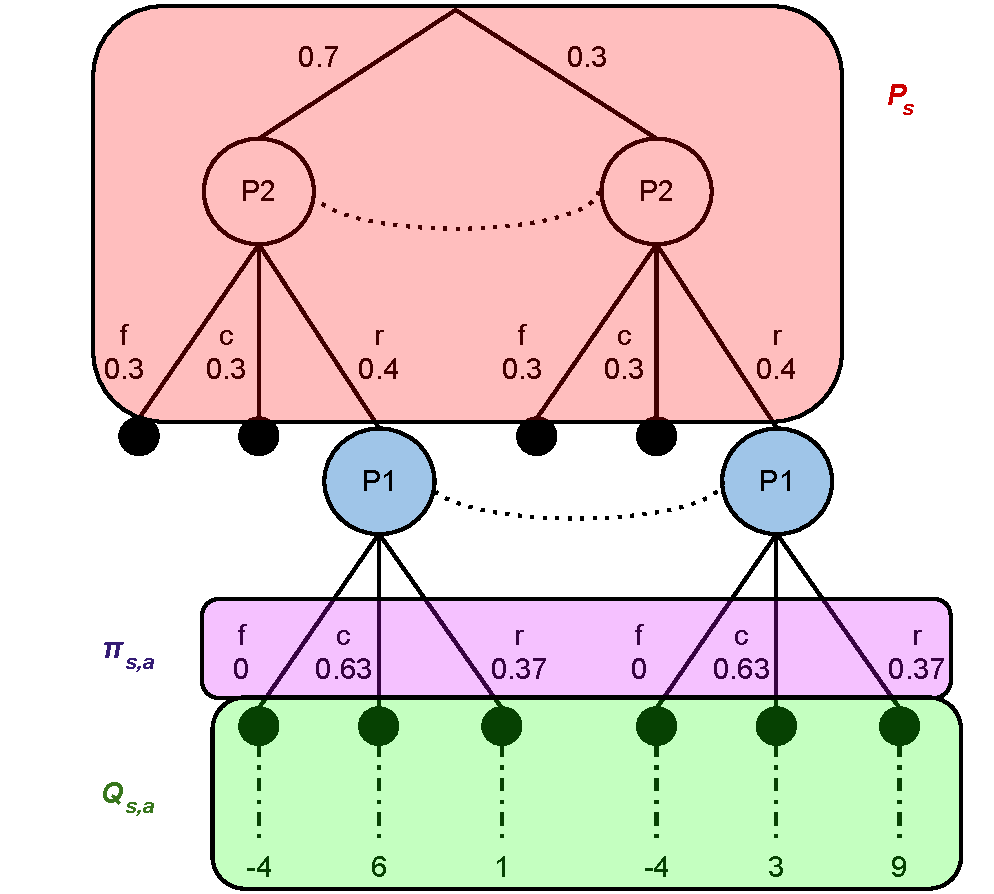
\includegraphics[scale=.5]{cfr_breakdown.pdf}
      \caption{An illustration of how Counterfactual Regret Minimization can be cast as a dynamic programming algorithm and, consequently, transformed into a temporal difference (TD) learning algorithm. The probability distribution over the nodes before a given information set correspond to the transition function, $P$, for that information set; the value of taking a given action in a specific information set is the $Q$-value function; and the function mapping an information set to a probability distribution over actions is the policy function $\pi$.}
      \label{fig-tdcfr}
    \end{figure}

    \begin{algorithm}
    \caption{TD-CFR}
    \label{alg-tdcfr}
    \begin{algorithmic}[1]
    \STATE \textbf{Input:} exploration rate $\xi$, exploration decay $\gamma^{\xi}$, learning rate $\alpha$, learning rate decay $\gamma^{\alpha}$
    \STATE $\pi_0 \leftarrow$InitializePolicy()
    \STATE $\pi_{avg} \leftarrow \pi_0$
    \FORALL{$(s,a) \in S \times A$}
        \STATE $Q(s,a) \leftarrow r^{max}$
        \STATE $P(s,a,s') \leftarrow$equal probability
        \STATE $Regret(s,a) \leftarrow 0$
    \ENDFOR
    \STATE iteration count, $i \leftarrow 1$
    \LOOP
        \STATE episode history, $h \leftarrow \{\}$
        \STATE reach probability, $reach \leftarrow 1$
        \WHILE{$playing hand$}
          \STATE $s \leftarrow$ current information set
          \STATE $\pi_{i} \leftarrow$UpdatePolicy($Regret, s, reach, \pi_{i-1}$)
          \STATE $rand \leftarrow$uniform random $[0,1]$
          \IF{$rand < \xi$}
            \STATE $a \leftarrow$randomly selected action
            \STATE $h \leftarrow \{(s,a)\}$
          \ELSE
            \STATE $a \leftarrow$action sampled from $\pi_i$
            \STATE $h \leftarrow h \cup (s,a)$
          \ENDIF
          \STATE $reach \leftarrow reach \times \pi_i(s,a)$
          \STATE $ev \leftarrow$ExpectedValue(Q,s)
          \STATE UpdateRegret($Regret,s,a,reach,ev,Q$)
          \STATE $i \leftarrow i+1$
        \ENDWHILE
        \FORALL{$(s,a) \in h$}
          \STATE $P \leftarrow$UpdateP($s,a,Q,\alpha$)
          \STATE $Q \leftarrow$UpdateQ($s,a,Q,\alpha$)
        \ENDFOR
        \STATE $\xi \leftarrow \xi \times \gamma^{\xi}$
        \STATE $\alpha \leftarrow \xi \times \gamma^{\alpha}$
    \ENDLOOP
    \end{algorithmic}
    \end{algorithm}

    \begin{algorithm}
    \caption{UpdatePolicy}
    \label{alg-tdcfr-updatepolicy}
    \begin{algorithmic}[1]
    \STATE \textbf{Input:} total counterfactual regret $Regret$, information set $s$, reach probability $reach$, current policy $\pi_{i-1}$, iteration $i$
    \STATE $R^{prev} \leftarrow Regret(s)$
    \STATE $R^{prev,+} \leftarrow$positive previous regret
    \STATE $probs \leftarrow$probabilities proportional to $R^{prev,+}$
    \STATE $\pi_{i} \leftarrow \pi_{i-1,-s} \cup (s,probs)$
    \STATE $\pi_{avg} \leftarrow \frac{1}{i} ((i-1)\times \pi_{i-1} + reach \times \pi_i)$
    \STATE return $\pi_{i}$
    \end{algorithmic}
    \end{algorithm}

    \begin{algorithm}
    \caption{UpdateRegret}
    \label{alg-tdcfr-updateregret}
    \begin{algorithmic}[1]
    \STATE \textbf{Input:} total counterfactual regret $Regret$, information set $s$, reach probability $reach$, selected action $a_{chosen}$, expected value $ev$, value function $Q$
    \FORALL{$a_{i}$ in $A(s)$}
        \STATE $cfr \leftarrow Q(s,a_{i}) - ev$
        \STATE $Regret(s,a_{i}) \leftarrow Regret(s,a_{i}) + cfr$
    \ENDFOR
    \end{algorithmic}
    \end{algorithm}

    \subsection{Policy Bootstrapping}
    Standard explicit modeling often takes a large number of samples to produce an effective counter-strategy, as it requires maintaining independent prior distributions at every information set in the opponent model. However, once the model has been learned, it can be used to generate a best response or repeatedly sampled to produce variants of the same type of opponent. Thus, if an explicit model could be efficiently learned, it could potentially be used to generate more robust responses than a simple implicit modeling agent. Obtaining the benefits of a generative opponent model with the quickness of an implicit model is the main motivating benefit behind the \textit{policy bootstrapping} algorithm.

    \begin{algorithm}
    \caption{Policy Bootstrapping}
    \label{alg-policybootstrapping}
    \begin{algorithmic}[1]
    \STATE \textbf{Input:} portfolio of strategies $\mathcal{S}$, initial strategy $s_0$
    \STATE $\mathcal{M} \leftarrow$InitializeOpponentModel($s_0$)
    \STATE $m \leftarrow$ImportanceSampling($\mathcal{M}$)
    \STATE $s \leftarrow$BestResponse($m$)
    \FORALL{$s_i \in \mathcal{S}$}
        \STATE $p(s_i) \leftarrow 1$
    \ENDFOR
    \LOOP
        \WHILE{$playing hand$}
            \STATE $I \leftarrow$current information set
            \STATE $a \leftarrow$ImportanceSampling($s(I)$)
            \STATE take action $a$
            \STATE $h \leftarrow h$ $\cup $ next opponent action
        \ENDWHILE
        \IF{opponent hand revealed}
            \FORALL{$s_i \in \mathcal{S}$}
              \STATE $p(s_i) \leftarrow p(s_i) \times p(outcome | s_i)$
            \ENDFOR
        \ELSE
            \FORALL{$s_i \in \mathcal{S}$}
              \STATE $x_{marg} \leftarrow 0$
              \FORALL{possible opponent holecards $hc$}
                \STATE $x_{marg} \leftarrow x_{marg} + p(outcome | s_i, hc)$
              \ENDFOR
              \STATE $p(s_i) \leftarrow p(s_i) \times x_{marg}$
            \ENDFOR
        \ENDIF
        \STATE $s_p \leftarrow$ImportanceSampling($\mathcal{S}$)
        \STATE $\mathcal{M} \leftarrow \mathcal{M} + s_p$
        \STATE $m \leftarrow$ImportanceSampling($\mathcal{M}$)
        \STATE $s \leftarrow$BestResponse($m$)
    \ENDLOOP
    \end{algorithmic}
    \end{algorithm}

    Algorithm \ref{alg-policybootstrapping} shows the policy bootstrapping algorithm in detail. A portfolio of precomputed opponent models, such as those used for implicit modeling, are given as input to the algorithm. Line 2 initializes an explicit opponent model using a baseline strategy, such as a uniform probability distribution or Nash equilibrium. The algorithm then performs importance sampling at every information set in the opponent model on line 3 to sample a single opponent strategy for exploitation. The best response to the sampled strategy is then played for one hand on lines 9-14. After the hand is complete, lines 15-28 update the pseudo-likelihood estimates for each of the portfolio models and performs importance sampling to choose a best-fit model for the next hand. The best-fit model's strategy is then added to the priors of the explicit opponent model in line 29, updating the beliefs about how the opponent behaves in a more sample efficient manner than direct updates which would only update the information sets along the observed trajectory.

    \subsection{Implicit Subpolicy Modeling}
    Rather than modeling a complete policy, either explicitly or implicitly, it may be more efficient to model components of an opponent's strategy. The key idea is that actions across various information sets are correlated, so when you see an example of an action in one information set, you can update your beliefs about other information sets. As an intuitive example, human players that are observed being aggressive when a specific draw is on the board in Texas Hold'em will likely also be aggressive when other similar draws are on the board, while it may reveal little about how they play in vastly different situations. Such correlations have been hypothesized previously in the literature \cite{bayesbluff,shortterm} and modeling opponents based on high-level features that discriminate situations based on the round and action has been used successfully in practice \cite{ponsen2009evolutionary}.\footnote{The notion of a subpolicy in this case is related to that of a feature set mapping to states. However, we separate the two concepts here as the distinction is important in subpolicy bootstrapping.} Thus, \textit{implicit subpolicy modeling} is presented as an approach to distinguish between the building blocks of an opponent's strategy. For all of our experiments, the implicit subpolicy modeling agent uses two subpolicies: preflop and flop actions.

    \subsection{Subpolicy Bootstrapping}
    Our final algorithm, \textit{subpolicy bootstrapping} combines explicit model bootstrapping with policy decomposition to yield an approach that weaves together an explicit opponent model from a set of subpolicies automatically discovered from a portfolio of complete strategies.

    Given a portfolio of strategies and a baseline strategy (e.g., a Nash equilibrium strategy), Algorithm \ref{alg-subpolicydiscovery} computes a set of subpolicies, where each subpolicy is applicable to some subset of the information sets in the opponent model. Lines 4-7 compute the deviation of the policy from the baseline strategy at information set as a proportion of the baseline strategy. For example, if the baseline strategy at a specific information set has the distribution $(0.1,0.5,0.4)$ and the portfolio policy has the distribution $(0.15, 0.4, 0.45)$, then the deviation at this information set is $(0.5, -0.2, 0.125)$. Lines 9-23 then perform a simple clustering of information sets based on \textit{L2}-distance.\footnote{The choice of clustering algorithms is arbitrary; other approaches such as k-means could also be used.} Lines 24-26 enforce a minimum size constraint on the subpolicies. Finally, on line 33 the algorithm returns the resulting set of all discovered subpolicies.

    \begin{algorithm}
    \caption{Subpolicy Discovery}
    \label{alg-subpolicydiscovery}
    \begin{algorithmic}[1]
    \STATE \textbf{Input:} portfolio of strategies $\mathcal{S}$, baseline strategy $s_b$, the minimum deviation $\delta_{min}$ from the baseline required to be a member of a subpolicy, the maximum deviation $\delta_{max}$ allowed from the centroid of a subpolicy to be considered a member, the minimum subpolicy size $size_{min}$
    \STATE $\Psi \leftarrow \{\}$
    \FORALL{$s_i \in \mathcal{S}$}
        \STATE $\mathcal{D} \leftarrow \{\}$
        \FORALL{information set $I$ in $s$}
            \STATE $\mathcal{D}_{I} \leftarrow s_i - s_b$
        \ENDFOR
        \STATE $\psi \leftarrow \{\}$
        \WHILE{$|\mathcal{D}| > 0$}
            \STATE $centroid \leftarrow \emptyset$
            \STATE $subpolicy \leftarrow \emptyset$
            \FORALL{$I,\mathcal{D}_I \in \mathcal{D}$}
                \IF{L2distance($\mathcal{D}_I$,$(0,0,0)$)$ < \delta_{min}$}
                    \STATE remove $I$ from $\mathcal{D}$
                \ELSIF{$centroid = \emptyset$}
                    \STATE $centroid \leftarrow \mathcal{D}_I$
                    \STATE $subpolicy \leftarrow \{(I,s_i(I))\}$
                    \STATE remove $I$ from $\mathcal{D}$
                \ELSIF{L2distance($\mathcal{D}_I,centroid$)$ < \delta_{max}$}
                    \STATE $subpolicy \leftarrow subpolicy \cup \{(I,s_i(I))\}$
                    \STATE remove $I$ from $\mathcal{D}$
                \ENDIF
            \ENDFOR
            \IF{$|subpolicy| > size_{min}$}
                \STATE $\psi \leftarrow \psi \cup subpolicy$
            \ENDIF
        \ENDWHILE
        \IF{$\psi = \emptyset$}
            \STATE $\psi \leftarrow s_i$
        \ENDIF
        \STATE $\Psi \leftarrow \Psi \cup \psi$
    \ENDFOR
    \STATE return $\Psi$
    \end{algorithmic}
    \end{algorithm}

    Once a set of subpolicies has been selected, either automatically or by hand, the subpolicy bootstrapping algorithm proceeds in a manner similar to that of full policy bootstrapping but with increased granularity and some statistical corrections to maintain the correct Bayesian priors. We refer the reader to our implementation for details on the main subpolicy bootstrapping algorithm.

\section{Experiments}
Experiments were performed on all four of our proposed algorithms and the standard approaches from the literature. We next detail our experimental setup and the results for each model in each experiment.

    \subsection{Setup}
    To analyze the performance of each model, we conducted a series of experiments in the game of Leduc poker. Leduc is a two-player poker variant where the deck contains six cards (two jacks, two queens, and two kings), each player is dealt a single hole card, there two rounds of betting, and a single community card is dealt after the first round. In total, Leduc contains 144 information sets for the second player, making this game non-trivial for agent modeling while still being tractable to analyze in-depth. For more information on Leduc poker, see \cite{bayesbluff}.

    \begin{figure}[thb]
      \centering
        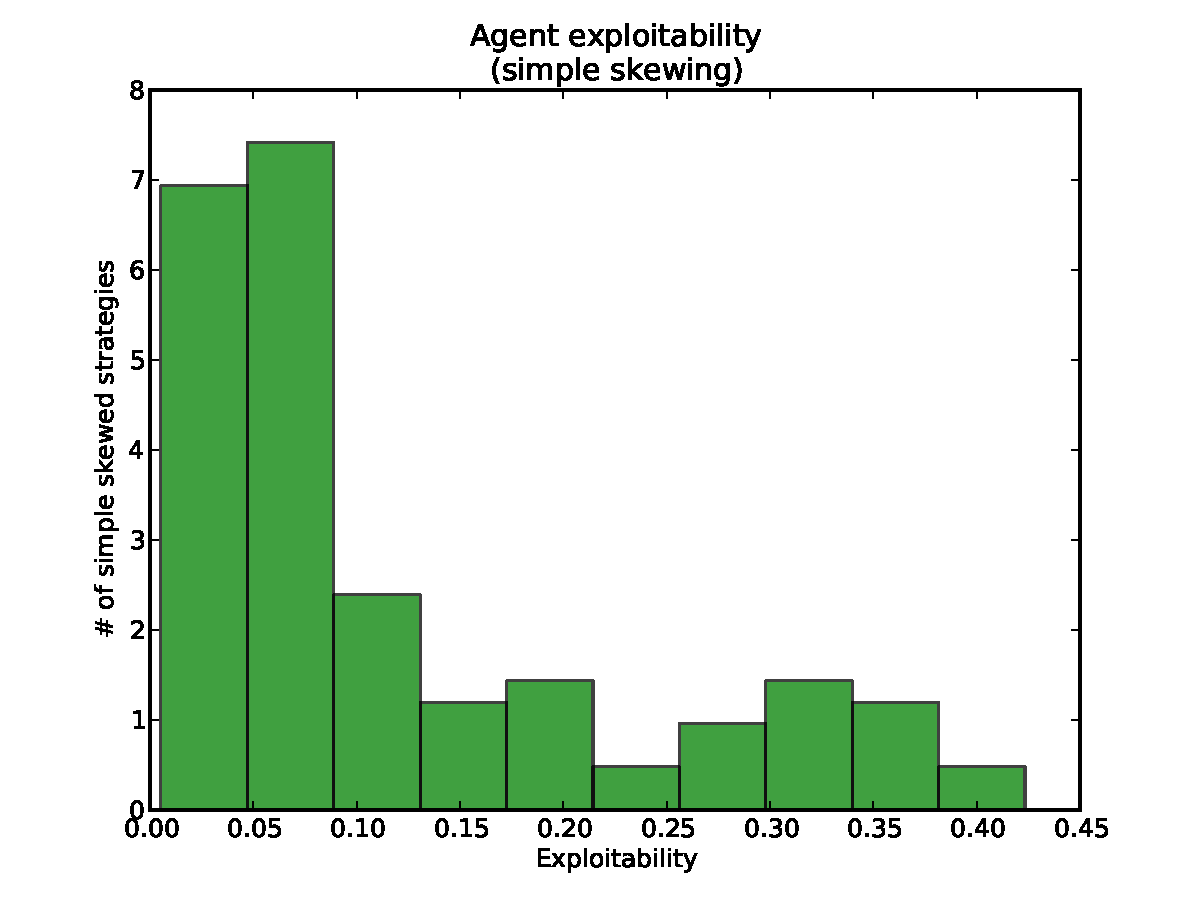
\includegraphics[scale=.45]{exploitability_simple.pdf}
      \caption{The maximum exploitability of the agents in the simple skewing population.}
      \label{fig-exploitability-simple}
    \end{figure}

    \begin{figure}[thb]
      \centering
        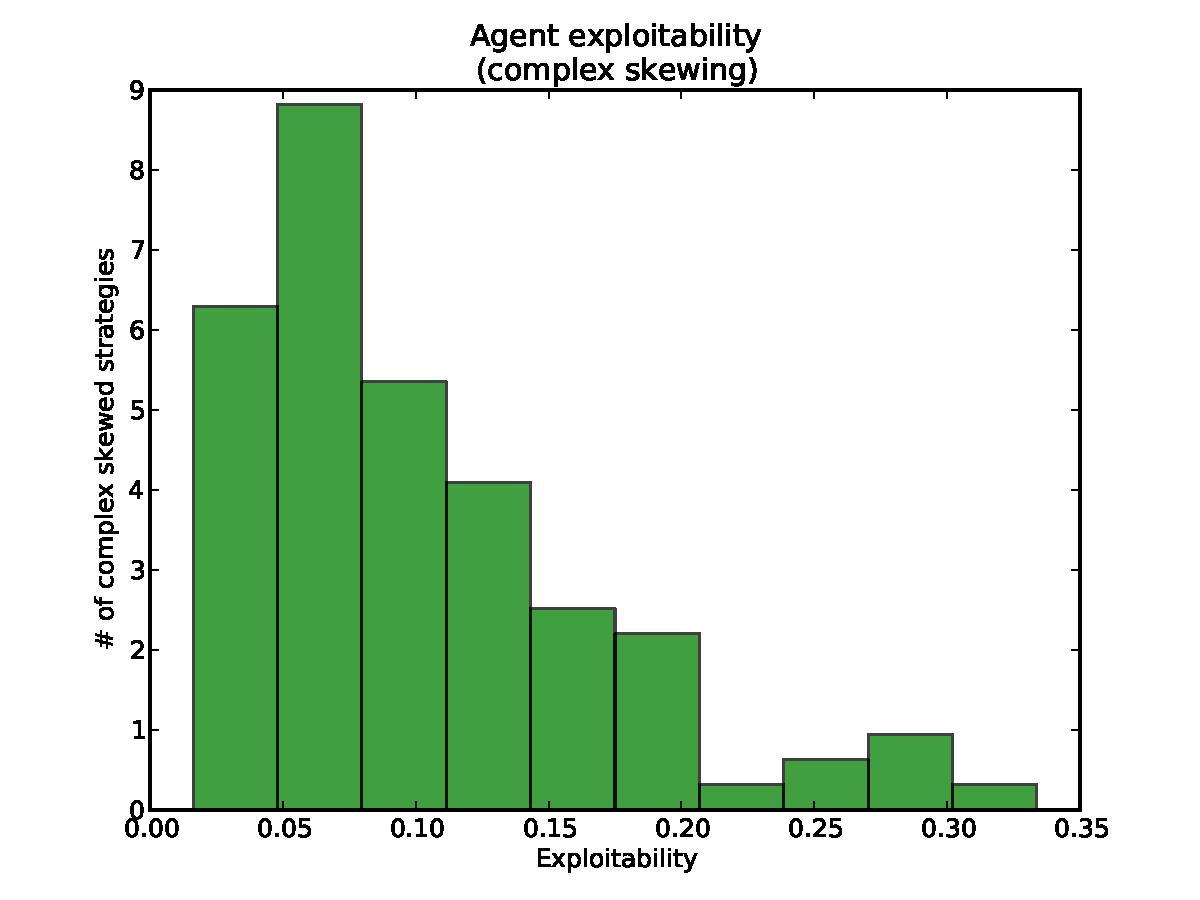
\includegraphics[scale=.45]{exploitability_complex.pdf}
      \caption{The maximum exploitability of the agents in the complex skewing population.}
      \label{fig-exploitability-complex}
    \end{figure}

    Experiments were conducted against three types of stationary opponents. First, a population of 100 ``simple'' agents was generated by generating two random percentage triplets for each agent; the first triplet was then used to skew the preflop actions of a Nash equilibrium strategy and the second was used to skew the flop actions. A population of 100 ``complex'' agents was then generated in a similar manner, where with equal probability the agent's preflop or flop actions were skewed, with a similar approach used to skew actions based on the holecard of the opponent (J, Q, or K). These two populations of agents aim to capture the systematic bias presumably found in human players that often over- or under- play a given hand or play looser or tighter at different points in the game. Finally, a Nash equilibrium strategy was used as a baseline to examine how the agents perform when trying to model an optimal player. Figures \ref{fig-exploitability-simple} and \ref{fig-exploitability-complex} show the distribution of exploitability values for the simple and complex experiments, respectively, setting an upper bound on how well an agent could perform against them in theory.

    In each experiment, the algorithms were tested for 200 matches of 200 hands each, with each algorithm playing against each simple and complex opponent twice. The TD-CFR agent used $\xi=0.1$ with an exponential $\xi$-decay factor of $0.99$ and a learning rate of $\alpha=0.05$. For portfolio-based methods, the portfolio consisted of the Nash equilibrium strategy and four skewed strategies, chosen at random from the population at the start of each match. For explicit models, two times the Nash strategy was used as an initial prior. The subpolicy discovery algorithm used the Nash equilibrium strategy as the baseline method, $\delta_{min}^{b}=0.05$, $\delta_{max}^{sp_i}=0.1$, and a minimum subpolicy size of 3.

    \subsection{Results}
    \label{sec-results}
    Figures \ref{fig-exploitedsimple} and \ref{fig-exploitedcomplex} show the results of the five approaches against the simple and complex skewed opponents, respectively. Note that in all cases, the TD-CFR results have been omitted as they performed too poorly to be plotted on the same graph without sacrificing the resolution of the other approaches. We refer the reader to the appendix for the graphs that include the TD-CFR results.

    The two implicit modeling approaches appear to perform the best, achieving the highest expected exploitation at nearly every step. Interestingly, the bootstrapped explicit model is able to approach approximately the same level as the implicit models by the end of the run, suggesting that bootstrapping an explicit model may be a viable approach to speeding up generative model learning. Unfortunately, subpolicy bootstrapping fails to perform as well as the other three novel approaches.

    Figure \ref{fig-exploitednash} presents the results of the six approaches against a Nash equilibrium player. Note that these learning curves are much smoother since each of the 200 trials is against the same opponent, reducing the variance in the evaluation process. Again, we see the two implicit modeling approaches performing strongest, with the bootstrapping methods approaching them in the end. 

    \begin{figure}[thb]
      \centering
        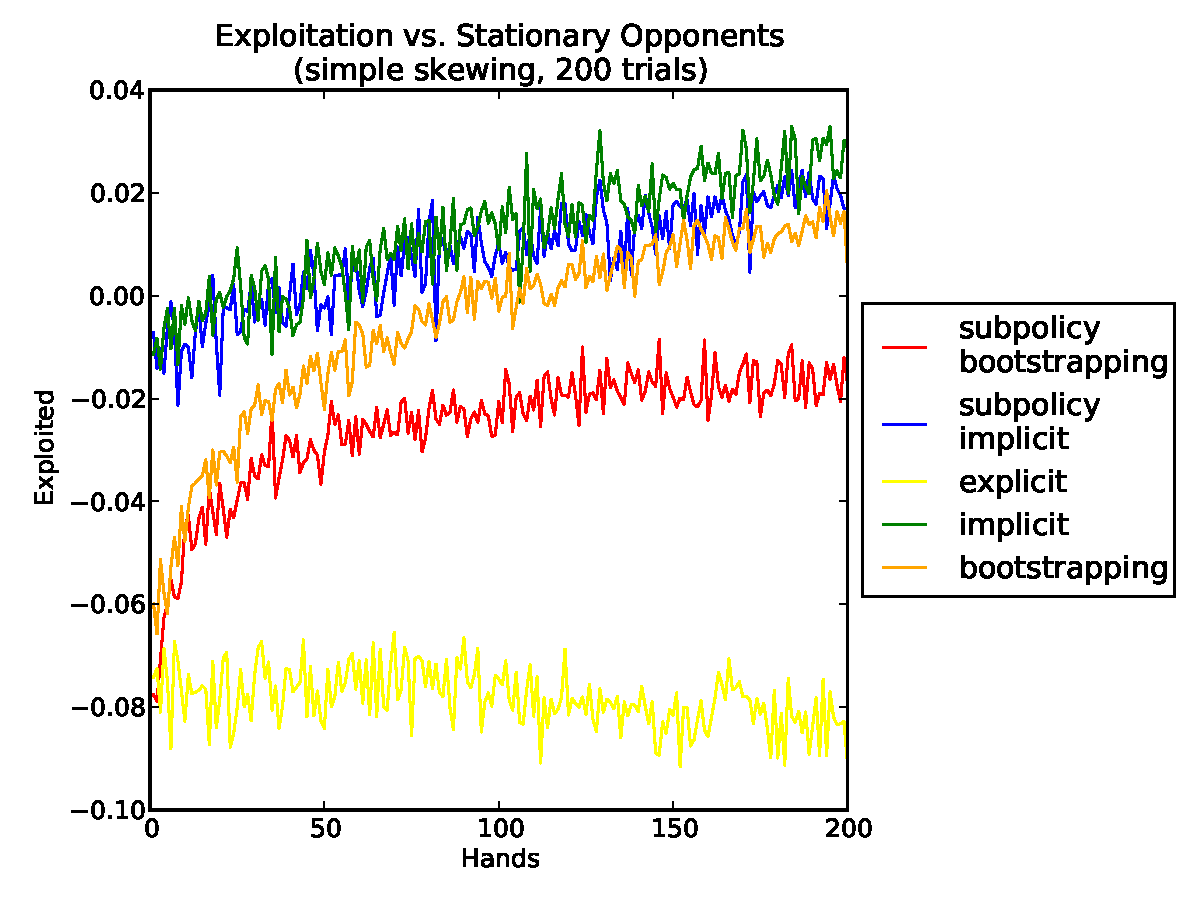
\includegraphics[scale=.45]{exploited_simple.pdf}
      \caption{The average performance of each algorithm against the population of exploitable agents derived from a simple strategy skewing methodology. Note that values near each other are not statistically significant due to overlapping confidence intervals.}
      \label{fig-exploitedsimple}
    \end{figure}

    \begin{figure}[thb]
      \centering
        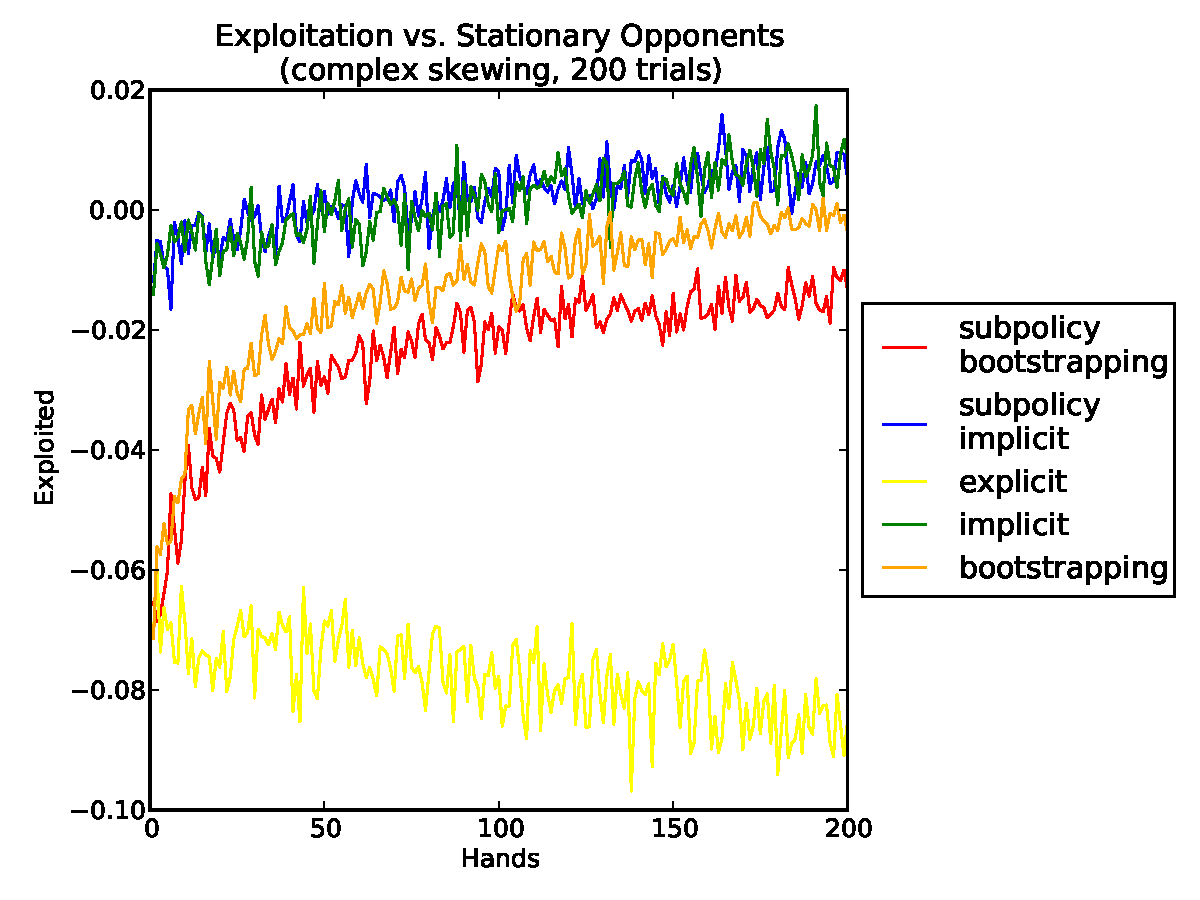
\includegraphics[scale=.45]{exploited_complex.pdf}
      \caption{The average performance of each algorithm against the population of exploitable agents derived from a relatively complex strategy skewing methodology. Note that values near each other are not statistically significant due to overlapping confidence intervals.}
      \label{fig-exploitedcomplex}
    \end{figure}

    \begin{figure}[thb]
      \centering
        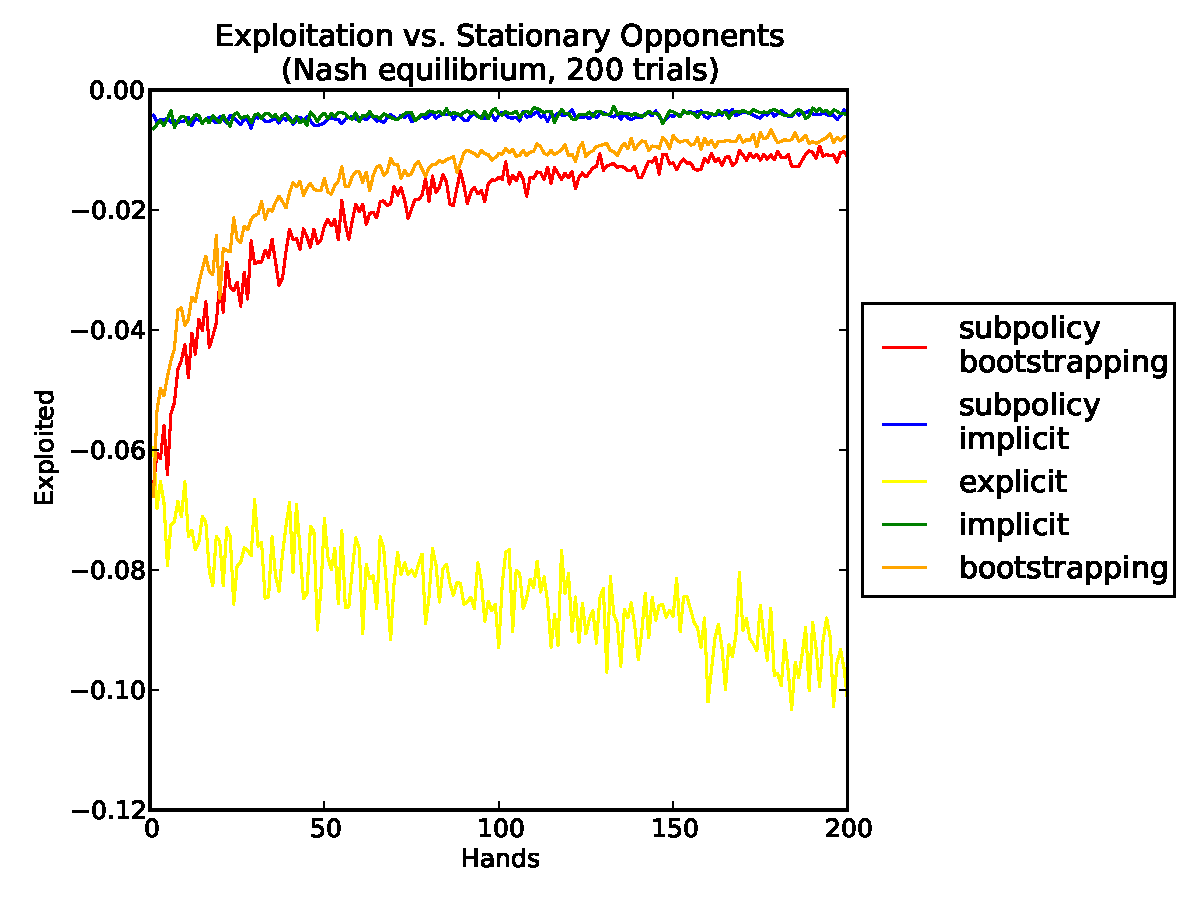
\includegraphics[scale=.45]{exploited_nash.pdf}
      \caption{The average performance of each algorithm against a Nash equilibrium agent.}
      \label{fig-exploitednash}
    \end{figure}


\section{Discussion}
The results of the three Leduc poker experiments raise interesting questions regarding the performance of each of the four novel methods relative to the benchmark approaches. We next discuss possible reasons for the performance of each model and speculate about the general potential of each approach.

The TD-CFR model, not shown in the performance figures due to its poor performance, shows little potential for improvement. Typically, we are concerned with one of two situations in poker: computing a strong strategy offline or adapting to exploitable opponents online. In the case of the former, direct methods like vanilla CFR or MC-CFR are likely more efficient than the TD-CFR approach. On the other hand, the CFR-inspired approach of TD-CFR makes for slow adaptation that can take hundreds of thousands of games to reach a good policy. Thus, the TD component of TD-CFR makes it ineffective for offline use and the CFR component makes it ineffective for online use, producing a method that unfortunately inherits the worst aspects of both approaches.

The policy bootstrapping results are possibly the most positive of all. Although not as efficient as implicit modeling in this domain, the ability of policy bootstrapping to quickly learn an explicit generative model suggests that it is a promising approach. It may be possible to start from a small portfolio of two or three models, play online against a new opponent, learn an explicit model of their play cheaply (or even profitably), and add the learned model into the portfolio for the next match. Such an approach could prove highly effective in real-world games where gathering a large portfolio directly would be prohibitively expensive.

Unfortunately, both implicit subpolicy modeling and subpolicy bootstrapping failed to outperform their complete policy counterparts. In the case of implicit subpolicy modeling, the performance is virtually identical, indicating that the potential gain for subpolicy modeling in Leduc may be too small to outweigh the increase in model complexity. To examine this possibility, we conducted experiments with 500 samples of randomly chosen implicit portfolios and opponents, where we measured the maximum exploitation of the opponent using the best response to each portfolio strategy, along with the maximum exploitation of the opponent using every possible subpolicy combination (using preflop and flop subpolicies) of the portfolio.

\begin{figure}[thb]
  \centering
    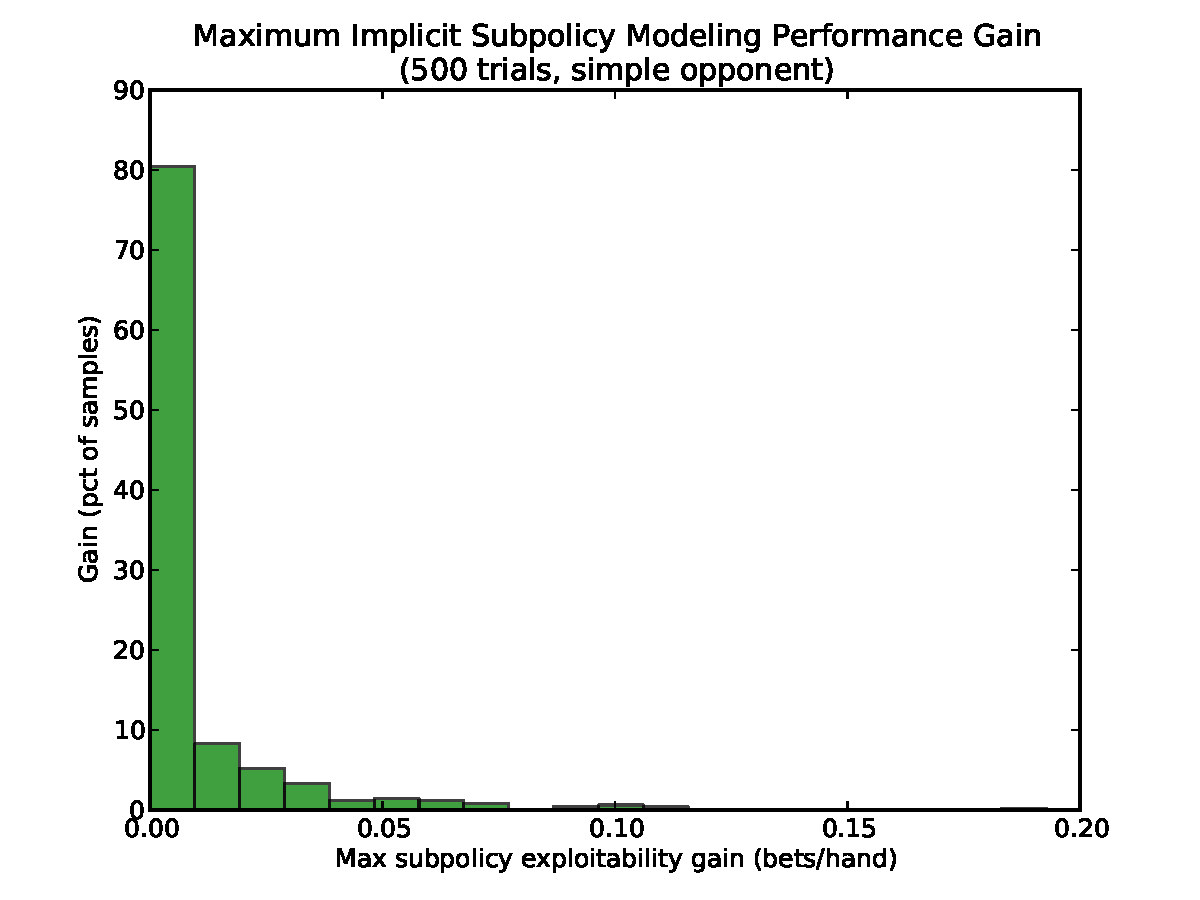
\includegraphics[scale=.4]{subpolicygain_simple.pdf}
  \caption{Results of 500 random trials calculating the maximum exploitation gain from using an implicit subpolicy approach instead of full policy implicit modeling. The vast majority of trials result in less than 0.01 bet/hand potential gain, indicating a possible reason for the failure of the implicit subpolicy modeling algorithm.}
  \label{fig-subpolicygain-simple}
\end{figure}

\begin{figure}[thb]
  \centering
    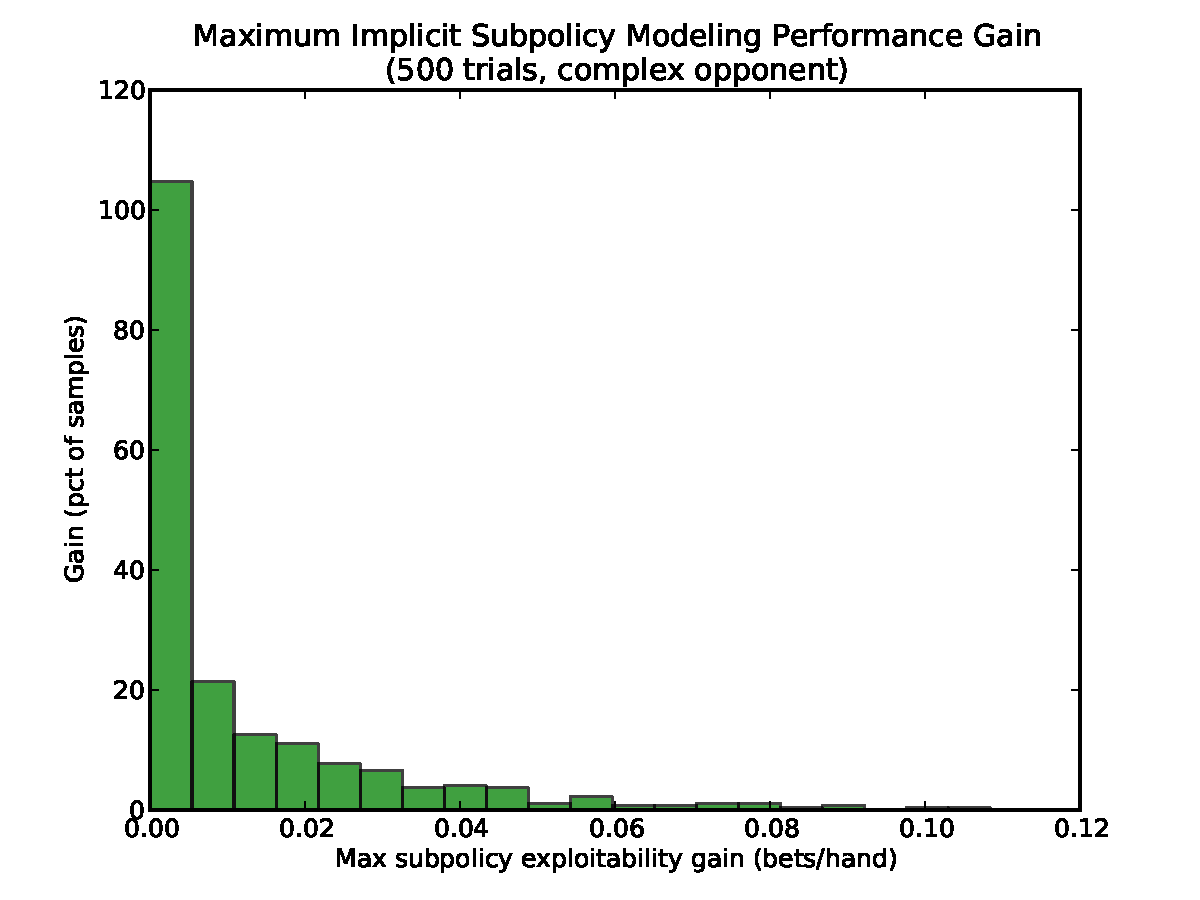
\includegraphics[scale=.4]{subpolicygain_complex.pdf}
  \caption{Results of 500 random trials calculating the maximum exploitation gain from using an implicit subpolicy approach instead of full policy implicit modeling. The vast majority of trials result in less than 0.01 bet/hand potential gain, further supporting the hypothesis that Leduc does not benefit from subpolicy modeling.}
  \label{fig-subpolicygain-complex}
\end{figure}

Figures \ref{fig-subpolicygain-simple} and \ref{fig-subpolicygain-complex} show the results of the experiment for the simple and complex skewing populations, respectively. In both cases, an overwhelming majority of the samples produced less than 0.01 bets-per-hand gain compared to the best complete policy response. Additionally, upon inspection of the game tree, only 9 information sets are contained in the preflop betting round as opposed to 135 for the flop round.\footnote{The flop betting round is also twice as expensive as the preflop round.} These results suggest that Leduc may generally be too small for round-based subpolicy partitioning. This may also help explain why subpolicy bootstrapping failed to outperform full policy bootstrapping.

\section{Future work}
The experiments conducted in this paper reveal several opportunities for future research. In this section, we highlight some of the areas that we believe are ripe for future work:

\begin{itemize}
\item \textbf{Learning opponent models from incomplete information.} Techniques like Data Biased Responses (DBRs) \cite{dbr} require a large number of well-chosen, perfect-information samples to form strong opponent models that can then be used online. In contrast, an approach like Deviation-Based Best Responses (DBBRs) \cite{dbbr} can potentially model opponents through incomplete information observations, but requires a startup phase of T hands to exploit an opponent. Ideally an exploitive agent would develop models that are both immediately exploitable and feasible to gather in practice.

\item \textbf{Increasing sample efficiency.} It seems intuitive that most real-world opponents' exploitable actions are correlated in a systematic way; this intuition has been noted by other researchers \cite{shortterm} as well. Increasing the information derived from opponent observations, whether from subpolicy analysis or some other approach, is critical to the success of future exploitive agent research.

\item \textbf{Subpolicy discovery.} Uncovering which subregions of opponent policies may contain the same systematic bias holds a large amount of potential. The straight-forward approach to subpolicy discovery through better feature engineering is a pragmatic approach, but a more general approach would be more powerful and be applicable to a wider class of games.

\item \textbf{Incremental best response calculation.} When maintaining an explicit opponent model where updates are made to only a portion of the model at each point, calculating a full best response may be unnecessary. In games such as Texas Hold'em, the full best response may be too computationally expensive to compute after every hand. An approach that can update only the parts of the model that are effected at each turn could vastly speed up the algorithm, with important practical implications.

\item \textbf{Modeling non-stationary opponents.} The vast majority of exploitive play in poker has assumed a stationary opponent, likely due to the presumed drastic increase in difficulty of opponent modeling. Fortunately, while this may be the case for game theoretic non-stationary agents, humans appear to use relatively simple models that are weighted heavily towards recent observations \cite{simplemodels}. Broadening the class of opponents to include such simple agents may hit the sweet spot of analytic tractability and real-world applicability.

\item \textbf{Deceptively teaching opponents.} All exploitive poker research to date has ignored the potential for teaching opponents an exploitable model. It seems reasonable that situations would present themselves, particularly against humans or agents using ``foresight-free'' models \cite{simplemodels}, where an agent could cheaply teach an opponent a policy that is exploitable for a much larger amount.
\end{itemize}

The above list has highlighted only some of the opportunities in the area of online opponent modeling. Given the small amount of research in the area, there may be numerous additional fruitful avenues of research.

\section{Conclusions}
This paper has presented four novel approaches to online opponent exploitation in poker. The TD-CFR method was proposed as a temporal difference learning variant of the CFR dynamic programming algorithm, and was found to perform poorly in all experiments. Three alternative, Bayesian approaches were then explored: policy bootstrapping, implicit subpolicy modeling, and subpolicy bootstrapping. None of these methods outperformed the standard implicit modeling benchmark, however policy bootstrapping was able to achieve significant speedups over direct explicit modeling. An in-depth study was conducted to determine the reason for the failure of the subpolicy methods and we concluded that Leduc may be too small of a test domain for such subpolicies to show any benefit, even when systematic biases are introduced into the opponents. We concluded with a list of potential areas for future work in opponent exploitation, in addition to exploring our four approaches on more challenging domains.

%
% The following two commands are all you need in the
% initial runs of your .tex file to
% produce the bibliography for the citations in your paper.
\bibliographystyle{abbrv}
\bibliography{sigproc}  % sigproc.bib is the name of the Bibliography in this case
% You must have a proper ".bib" file
%  and remember to run:
% latex bibtex latex latex
% to resolve all references
%
% ACM needs 'a single self-contained file'!
%
%APPENDICES are optional
%\balancecolumns
\appendix

\section{TD-CFR Results}
The graphs from section \ref{sec-results} omitted the TD-CFR results so as to enable better presentation of the other methods. For completeness, we include the full graphs here.

\begin{figure}[tbh]
\centering
  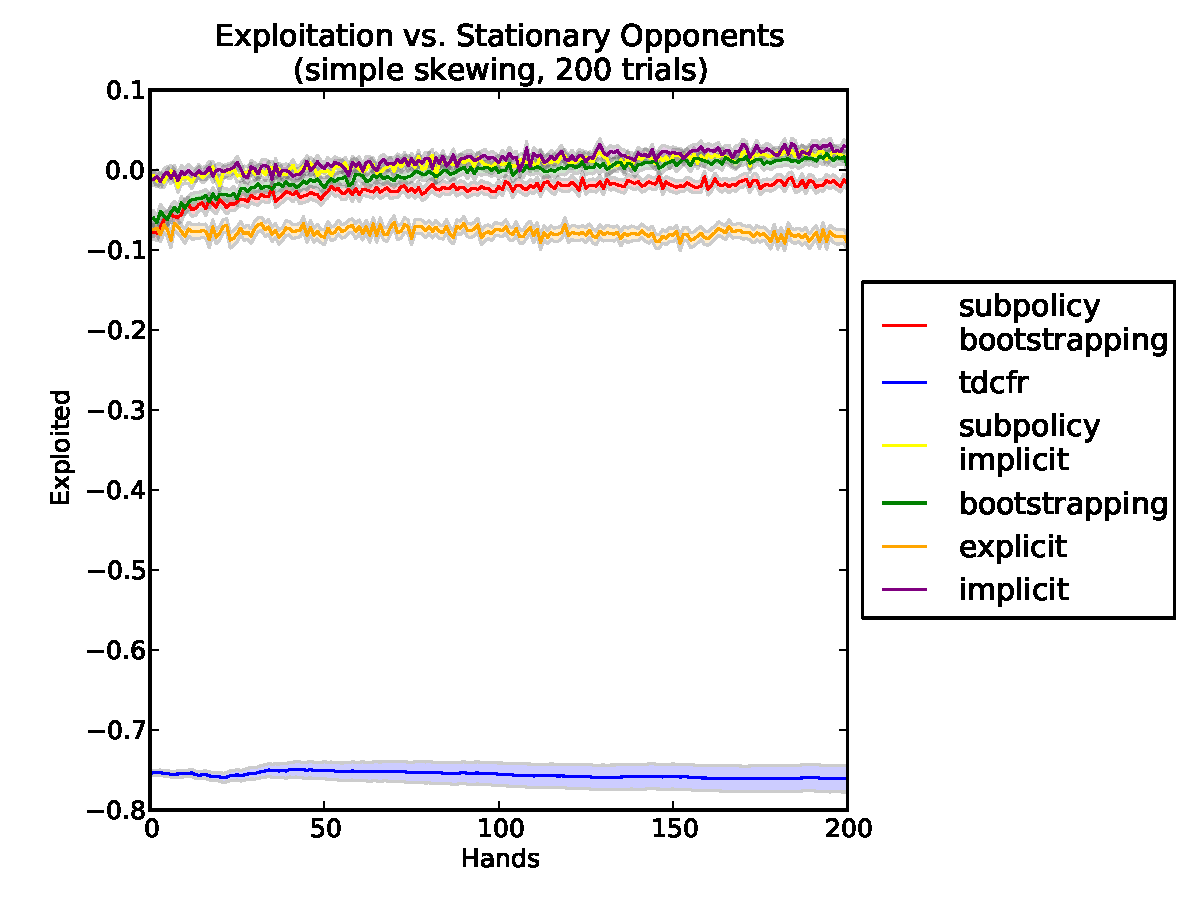
\includegraphics[scale=.4]{exploited_simple_tdcfr.pdf}
\caption{The average performance of each algorithm against the population of exploitable agents derived from a simple strategy skewing methodology.}
\label{fig-exploitedsimple-tdcfr}
\end{figure}

\begin{figure}[tbh]
\centering
  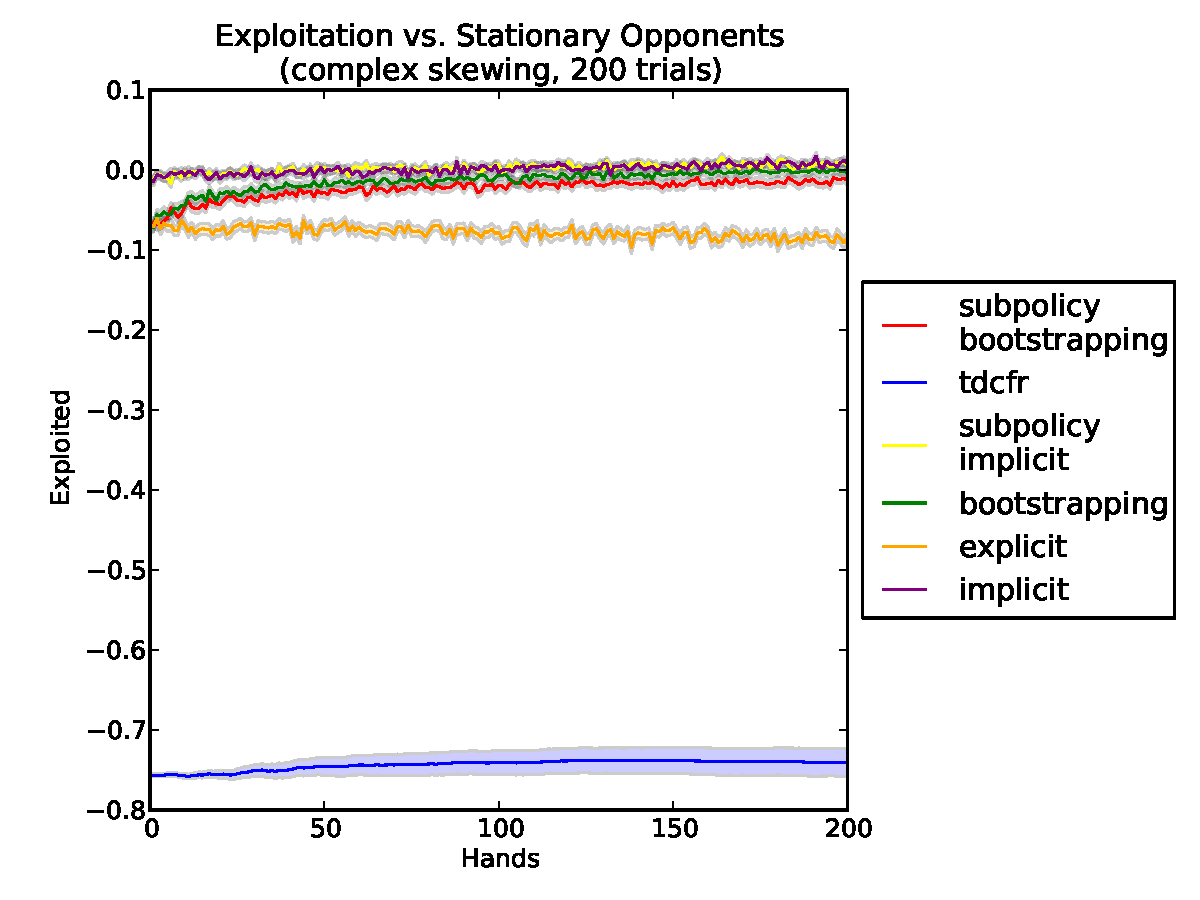
\includegraphics[scale=.4]{exploited_complex_tdcfr.pdf}
\caption{The average performance of each algorithm against the population of exploitable agents derived from a relatively complex strategy skewing methodology.}
\label{fig-exploitedcomplex-tdcfr}
\end{figure}

\begin{figure}[tbh]
\centering
  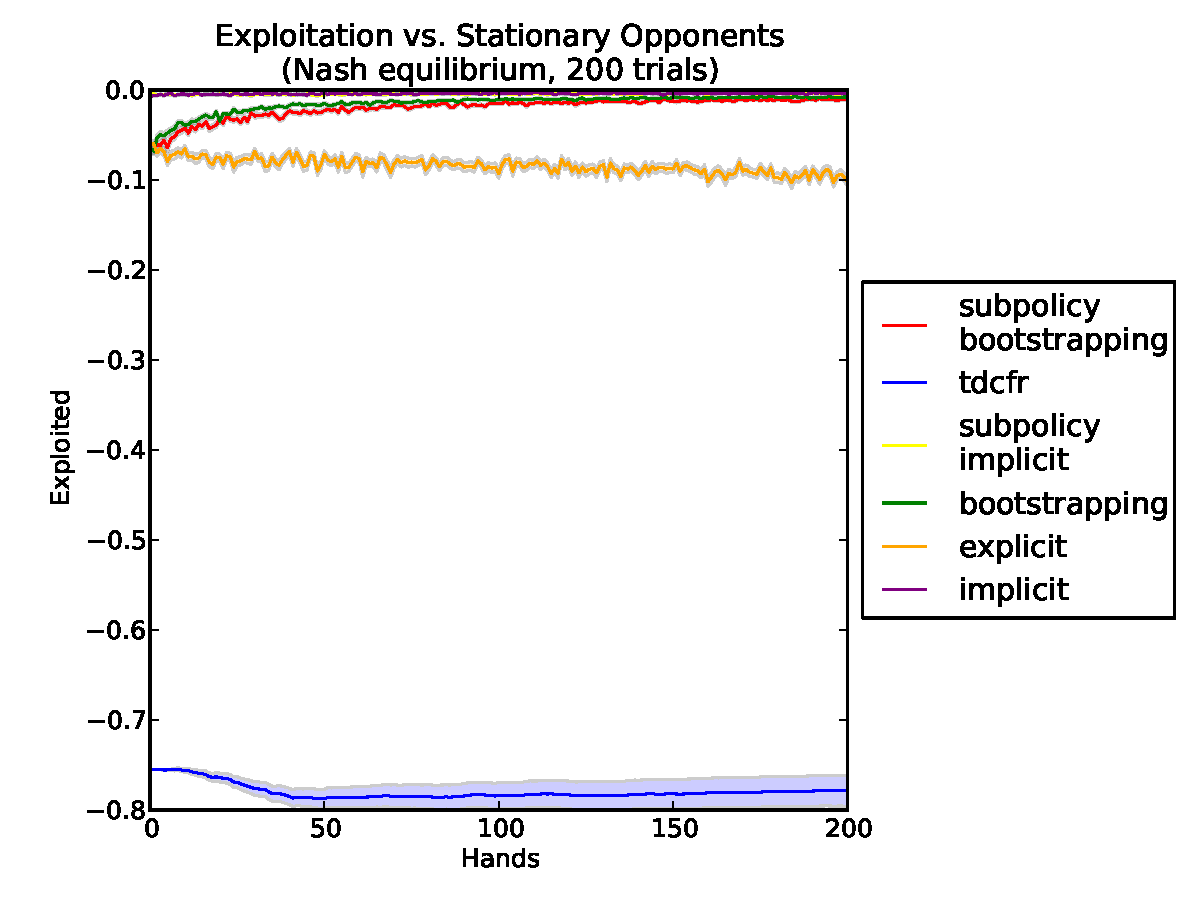
\includegraphics[scale=.4]{exploited_nash_tdcfr.pdf}
\caption{The average performance of each algorithm against a Nash equilibrium agent.}
\label{fig-exploitednash-tdcfr}
\end{figure}

\section{Confidence Intervals}

Due to the large number of time series, confidence intervals were left off of the graphs in section \ref{sec-results}. For completeness, we include them here.

\begin{figure}[tbh]
\centering
  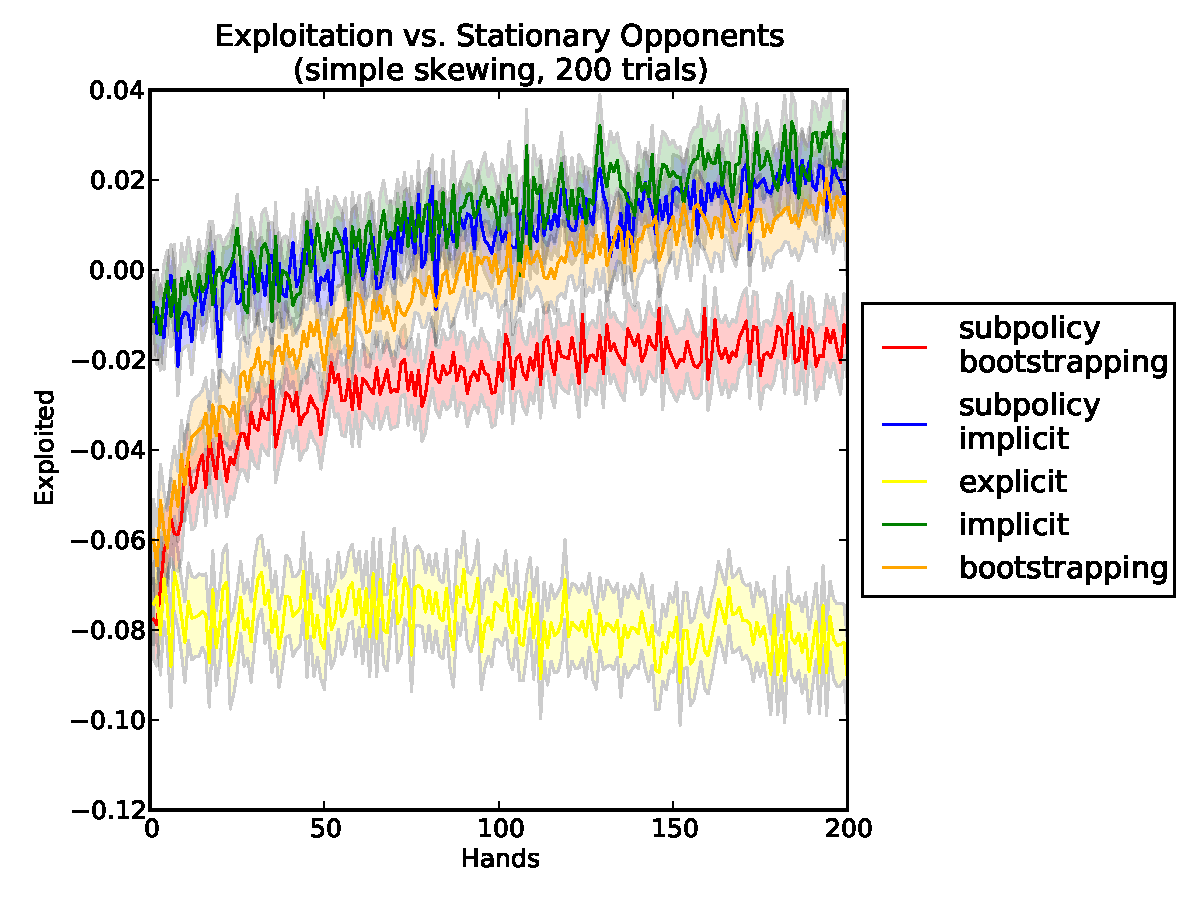
\includegraphics[scale=.4]{exploited_simple_confidence.pdf}
\caption{The average performance of each algorithm against the population of exploitable agents derived from a simple strategy skewing methodology.}
\label{fig-exploitedsimple-confidence}
\end{figure}

\begin{figure}[tbh]
\centering
  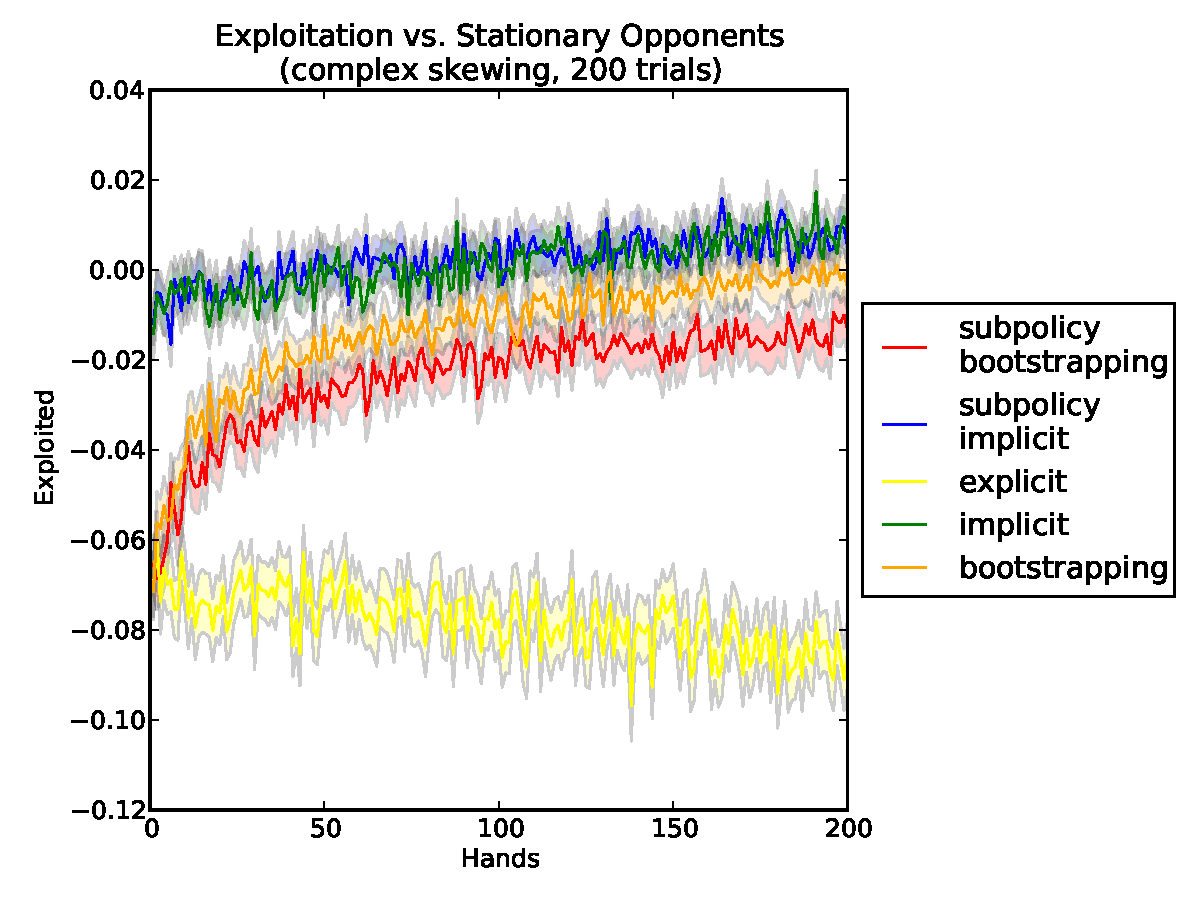
\includegraphics[scale=.4]{exploited_complex_confidence.pdf}
\caption{The average performance of each algorithm against the population of exploitable agents derived from a relatively complex strategy skewing methodology.}
\label{fig-exploitedcomplex-confidence}
\end{figure}

\begin{figure}[tbh]
\centering
  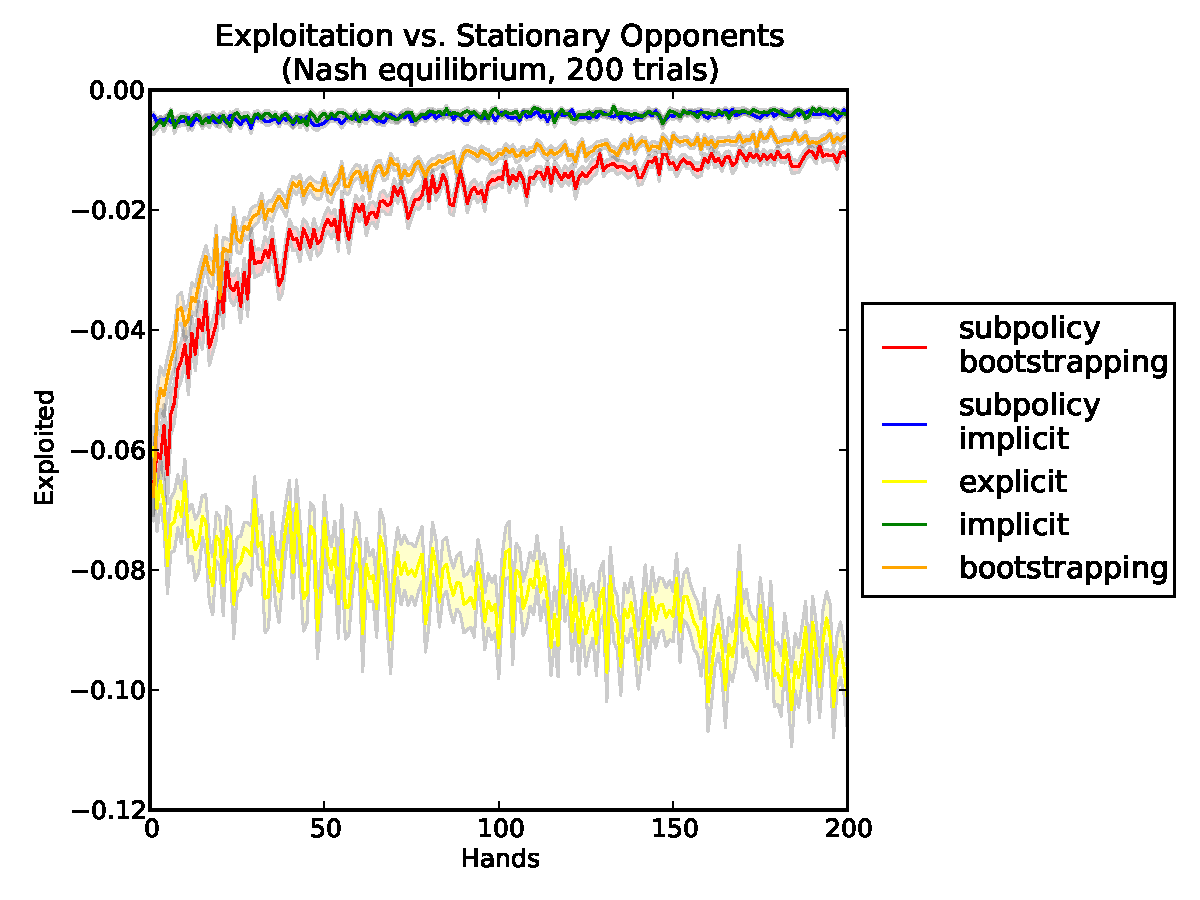
\includegraphics[scale=.4]{exploited_nash_confidence.pdf}
\caption{The average performance of each algorithm against a Nash equilibrium agent.}
\label{fig-exploitednash-confidence}
\end{figure}

%\balancecolumns % GM June 2007
% That's all folks!
\end{document}
